\documentclass[10pt]{article}

\usepackage[letterpaper]{geometry}
\usepackage{color}
\usepackage{hyperref}
\usepackage{fancyhdr}
\usepackage{sectsty}
\usepackage{amsmath}
\usepackage{graphicx}
\usepackage{pdflscape}

\setlength{\headheight}{0pt}
\setlength{\headwidth}{6.5in}
%\pagestyle{fancy}

\setlength{\textwidth}{6.5in}
\setlength{\textheight}{8.5in}
\setlength{\topmargin}{0in}
\setlength{\oddsidemargin}{0.0in}
\setlength{\evensidemargin}{0.0in}
\setlength{\rightmargin}{0.0in}
\setlength{\footskip}{.5in}
\setlength{\parindent}{0pt}

\newcommand{\angstrom}{\text{\normalfont\AA}}
\newcommand{\blankline}{\quad\pagebreak[3]}
\sectionfont{\fontsize{13}{15}\selectfont}


\linespread{1.07}

\title{\Large{\bf EUVICS}: \\
        \Large{\bf An Accelerator-Based EUV Light Source  \\
        Using the Inverse Compton Scattering
}}
        
\author{\large Chong Shik Park, Ph.D, \\
Korea University, Sejong 30019, South Korea}

\begin{document}

\maketitle

\tableofcontents
%\tableofcontents

%\newpage
%\begin{landscape}
%\null
%\vfill
%\begin{figure}[ht]
%  \centering
%    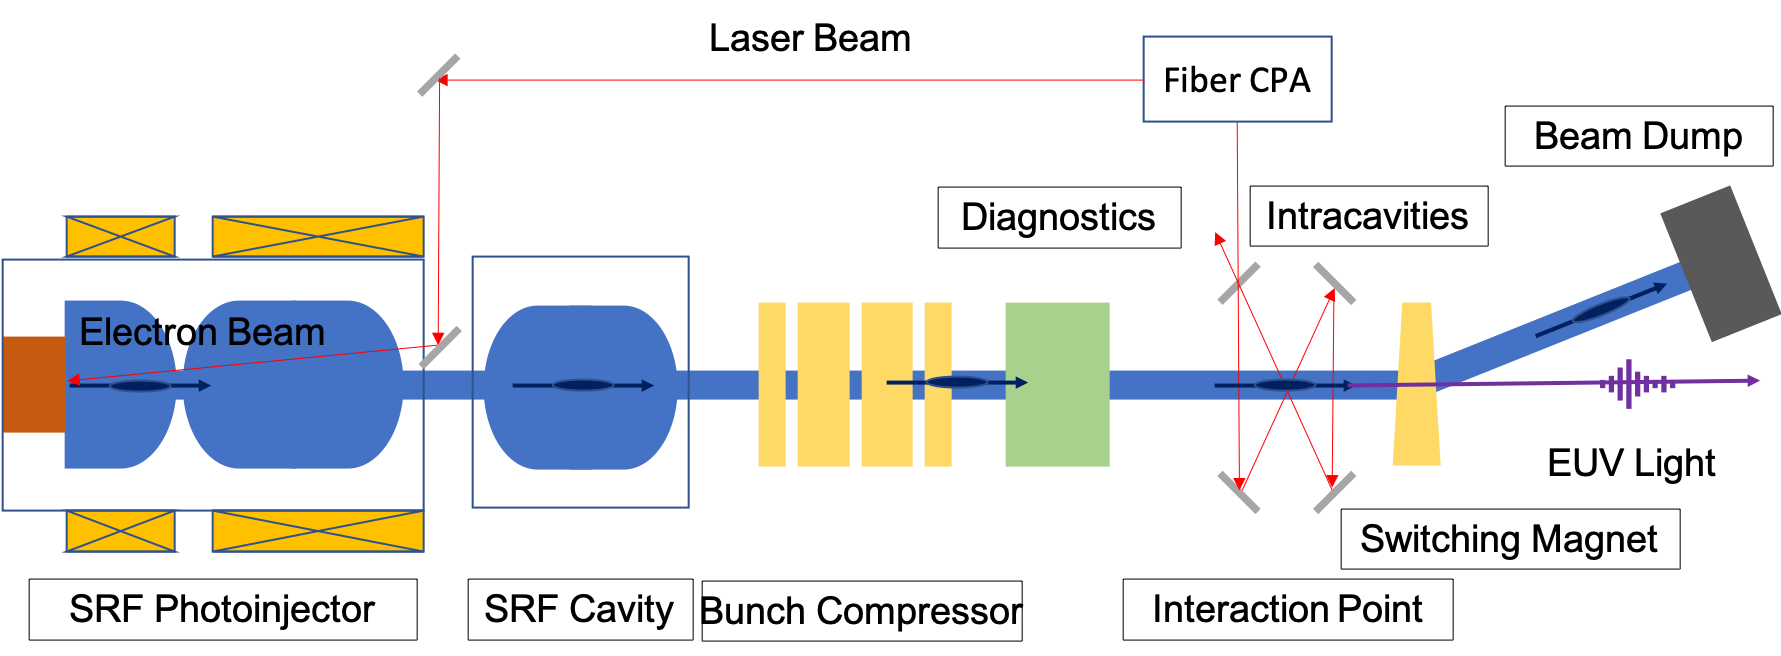
\includegraphics[width=8in]{img/ics-layout.png}
%    \caption{Inverse Compton Scattering EUV Light Source Layout}
%    \label{fig:layout}
%\end{figure}
%\vfill
%\end{landscape}

\newpage

\section{Introduction}

  \subsection{EUV Light Source Design Criteria}
  
  The design of an Extreme Ultraviolet (EUV) light source must meet stringent criteria to ensure its suitability for applications such as advanced lithography, materials science, and other high-precision technologies. Key criteria include high brightness, narrow bandwidth, and stability of the EUV output, along with efficiency and reliability of the overall system. Additionally, the system must be designed to minimize operational costs and ensure ease of maintenance and scalability for future enhancements.
  
  \subsection{Accelerator-Based EUV Light Sources}
  
  Accelerator-based EUV light sources leverage the high-energy electrons generated by particle accelerators to produce EUV radiation. These sources typically offer higher brightness and better control over beam parameters compared to plasma-based sources. The integration of advanced accelerator technologies, such as superconducting RF linacs and photoinjectors, enables the production of highly collimated, high-intensity EUV beams, which are essential for next-generation lithography and other cutting-edge applications.
  
  \subsection{ICS EUV Light Source Design Concept and Performance Goal}
  
  The design concept for an ICS-based EUV light source involves the interaction of a high-energy electron beam with a high-power laser beam to produce EUV photons through Inverse Compton Scattering. The performance goal is to achieve a high-brightness, narrow-bandwidth EUV output with excellent stability and efficiency. The system aims to provide an EUV source that meets the demanding requirements of industrial and scientific applications, offering a robust and scalable solution for future technological advancements.


\blankline
\blankline

\section{Overview of Inverse Compton Scattering EUV Light Source}

  \subsection{Physics of Inverse Compton Scattering}
  
  Inverse Compton Scattering (ICS) involves the interaction between high-energy electrons and photons, resulting in the photons being scattered to higher energies. This process is central to generating Extreme Ultraviolet (EUV) light for various applications. The relativistic electrons transfer energy to lower-energy photons, boosting them to the EUV range, which is crucial for advanced lithography and other technologies.
  
  
  \subsection{Accelerator System}
  
  The accelerator system is designed to produce a high-quality electron beam required for efficient ICS. It includes components such as the electron injector, superconducting RF linac, and beam transport system, which collectively ensure the generation and delivery of a stable, high-energy electron beam.
  
  
  \subsection{Laser System}
  
  The laser system provides the initial photons that interact with the electron beam in the ICS process. This system needs to deliver high-power, high-frequency laser pulses with precise timing and synchronization to achieve the desired EUV light production.
  
\blankline
\blankline
  
\section{Electron Injector - Superconducting RF Photoinjector}

  \subsection{Design Requirements}
  
  The electron injector must deliver a high-brightness, low-emittance electron beam with the necessary parameters for subsequent acceleration. This includes considerations for beam energy, current, and pulse structure.
  
  
  \subsection{Accelerator Physics Design}
  
  The design involves optimizing the injector's geometry and operational parameters to maximize beam quality. This includes simulations and modeling to achieve the required beam characteristics.
  
  
  \subsection{R\&D Required}  
  
  Research and development are needed to address technical challenges such as cavity design, cryogenic systems, and beam diagnostics. Innovations in superconducting materials and photoinjector technologies are critical for achieving the desired performance.
  

\blankline
\blankline

\section{Superconducting RF Linac}

  \subsection{Design Requirements}
  
  The RF linac must accelerate the electron beam to the energies required for effective ICS. Key requirements include high accelerating gradients, energy stability, and efficient cryogenic systems.
  
  \subsection{Accelerator Physics Design}
  
  Designing the linac involves detailed simulations to optimize the accelerating structures, beam dynamics, and overall system efficiency. This includes considerations for cavity design, RF power delivery, and beam transport.
  
  \subsection{R\&D Required}  
  
  R\&D efforts will focus on developing advanced superconducting cavities, improving RF power sources, and enhancing cryogenic technologies. Addressing these challenges is essential for reliable and efficient linac operation.
  

\blankline
\blankline

\section{Incident Laser System and Interaction Region}

  \subsection{Design Requirements}
  
  The incident laser system must produce high-power, short-duration pulses synchronized with the electron beam. The interaction region needs to facilitate optimal overlap between the electron and photon beams for efficient ICS.
  
  \subsection{Accelerator Physics Design}
  
  Designing this system involves optimizing laser parameters, synchronization mechanisms, and the geometry of the interaction region. Advanced diagnostics and feedback systems are also crucial for maintaining performance.
  
  \subsection{R\&D Required}  
  
  R\&D will focus on developing high-power laser sources, precision timing systems, and advanced optical components. Innovations in these areas will enhance the efficiency and reliability of the ICS process.

\blankline
\blankline

\section{System Integration and Control}

  \subsection{Design Requirements}
  
  System integration requires a comprehensive control system to manage the accelerator, laser, and interaction region components. This includes ensuring precise synchronization, stability, and safety.
  
  \subsection{Accelerator Physics Design}
  
  The control system design involves developing algorithms and hardware for real-time monitoring and adjustment of system parameters. This ensures optimal performance and addresses any deviations promptly.
  
  \subsection{R\&D Required}  
  
  R\&D efforts will be directed towards developing advanced control systems, integrating diagnostics, and enhancing user interfaces. These developments are crucial for the seamless operation of the entire EUV light source system.


\blankline
\blankline

\section{Cost Estimate}

  \subsection{Basis of Estimate}
  
  The cost estimate is based on detailed analyses of each system component, including materials, labor, and R\&D expenses. This includes benchmarking against similar projects and industry standards.
  
  \subsection{Cost Summary}
  
  The cost summary provides a breakdown of expenses for each major component and system. This includes the electron injector, RF linac, laser system, interaction region, and control systems. The summary also accounts for contingencies and potential cost variations.


%%%%%%%%%%%%%%%%%%%%%%%%%%%%%%%%%%%%%%%%%%%%%%%%%%%

%\begin{thebibliography}{77}
%
%  \raggedright
%
%  \bibitem{blahblah}
%  blahblah
%
%
%\end{thebibliography}

\end{document}
